\newcommand{\projectName}{Az EGTIB}

\chapter{\projectName{} bemutatása}

\projectName{} projekt célja egy olyan felhasználóbarát felület létrehozása, mely lehetőséget teremt a daganatos sejtek játékelméleti modellezésére és szimulációjára, a szimulációs eredmények megjelenítésére illetve ezeknek valamilyen szintű mentésére is. Ezért született meg, a mai trendeket figyelembe véve, egy kliens-szerver architektúrán alapuló webalkalmazás, mely részben az \cite{archetti2016cooperation}-ben megjelent modellt implementálja, és ahhoz új funkcionalitásokat is hozzáad.

\begin{figure}[ht!]
	\centering
	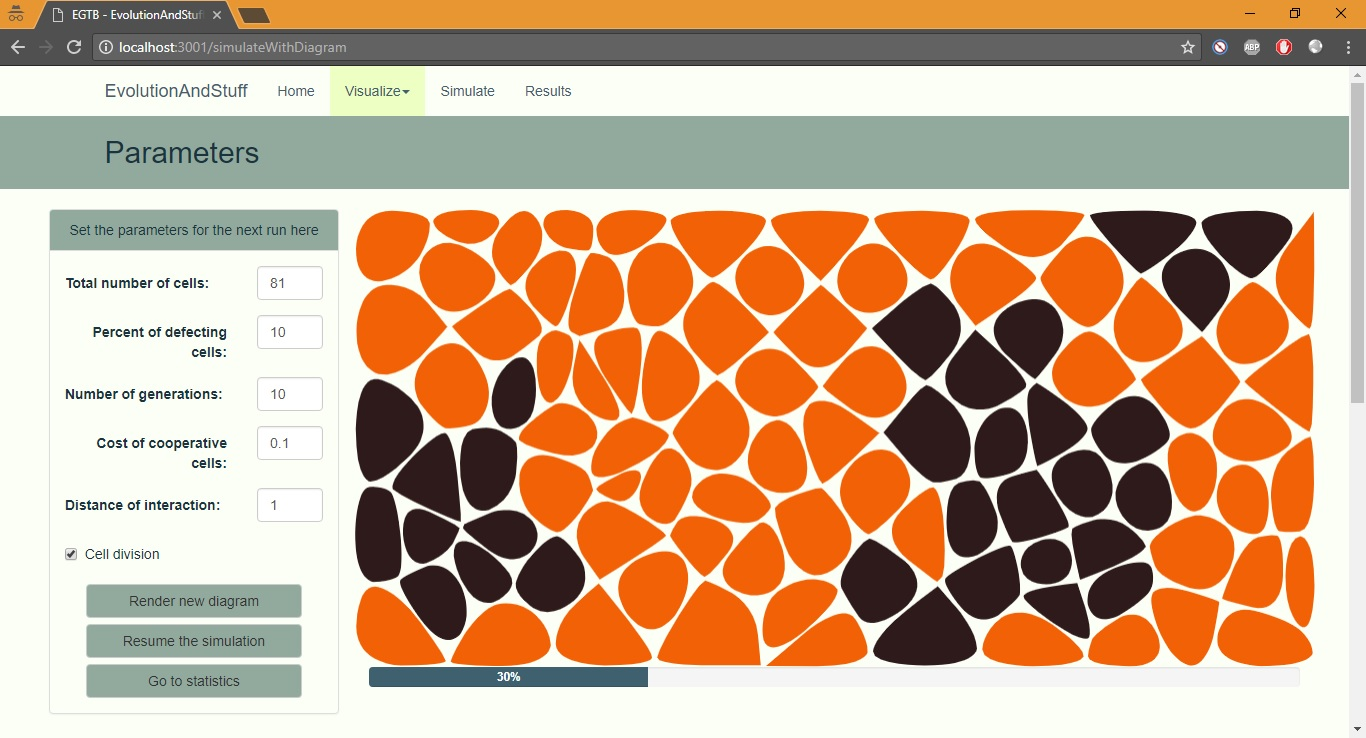
\includegraphics[width=90mm]{images/EGTIB}
	\caption{Pillanatkép az alkalmazásról \label{fig:SimulateWithDiagram}}
\end{figure}

\section{Funkcionalitások}

Az alkalmazásunkat, funkcionalitás szerint, három fő komponensre oszthatjuk:

\paragraph{Vizualizáció}- képes szimulálni kevés sejtből (max. 500) álló populációkat és ezeket generációnként meg is tudja jeleníteni. A megjelenítés interaktív, ami azt jelenti, hogy bármikor meg lehet állítani, folytatni vagy akár tekergetni mint egy filmet. Továbbá mindehhez tartozik egy grafikon is, mely a populációnak változását ábrázolja generációnként.

\paragraph{Szimuláció}- alkalmas nagyobb (max. 2000) populációval dolgozni, viszont ezek megjelenítése már túl sok időt venne igénybe, így csak a fentebb említett grafikon segítségével ábrázolja azt, hogy mi is történik a sejtek között. Előnye a vizualizációs részhez képest elsősorban az, hogy sokkal nagyobb populációval tud dolgozni, de a paraméterlista is változatosabb (a szimuláció során használt függvények viselkedésébe is bele tud szólni a felhasználó) és hatalmas kényelmi faktornak számít az, hogy több, különböző paraméterezésű szimulációt is képes egy gombnyomással lekérni.

Mindkét esetben a felhasználónak lehetősége van bizonyos paramétereket megválasztani még a szimulálási fázis előtt:
\begin{itemize}[noitemsep]
	\item kezdeti populáció mérete
	\item defektálók aránya 
	\item generáció szám (szimuláció hossza)
	\item kooperáló sejtek termelési költsége 
	\item diffúziós távolság mérete
	\item akarja-e a felhasználó, hogy a sejtek osztódásra legyenek képesek
\end{itemize}
Ezen paramétereket felhasználva kigenerálható egy Voronoi diagram mely a sejteket ábrázolja. A simulate gombot megnyomva ez az adatcsomag eljut a szerverhez amely elvégzi az erőforrás igényes számításokat melynek eredményét visszaküldi a kliensnek, ami majd azt megjeleníti.

Továbbá a szimulációs oldalon az alábbi paraméterek is változtathatóak:
\begin{itemize}[noitemsep]
	\item a V függvény meredeksége
	\item a V függvény áthajlási pontjának helye
	\item a gradiens alakja
	\item a gradiens meredeksége az áthajlási pontban
\end{itemize}
melyek segítségével a felhasználónak sokkal nagyobb beleszólása van abba, hogy a populáció hogyan is viselkedjen. Mivel ezek a felhasználónak csak puszta számok, elég nyers adat, így segítségére siet két grafikon (\ref{fig:SimulationFunctionDiagrams}), mely a paraméterlista mellett kapott helyet. Ezen grafikonokon a két függvény jelenítődik meg, melyek interaktívak, azaz az értékek változtatásával a grafikon is átalakul, így szemléltetve a felhasználó előtt, hogyan is néz ki az adott V (\ref{eq:payoffGradient}) illetve g (\ref{eq:diffGradient}) függvény.

\begin{figure}[ht!]
	\centering
	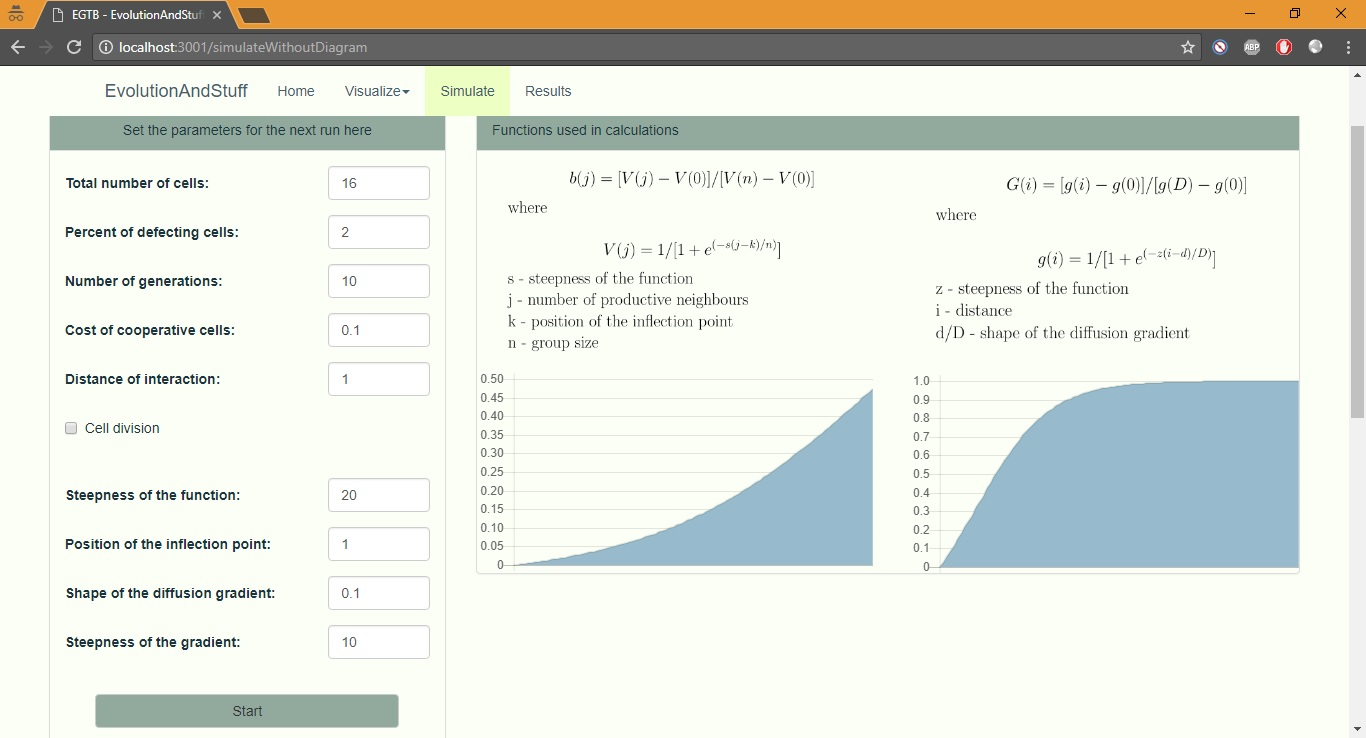
\includegraphics[width=90mm]{images/SimulationFunctionDiagrams}
	\caption{A V és g függvények alakja adott paraméterekre}
	\label{fig:SimulationFunctionDiagrams}
\end{figure}


\paragraph{Eredmények}- kezdetben már azzal is megelégedtünk, ha egy szimulációt képesek voltunk megjeleníteni, viszont egy idő után azt vettük észre, hogy milyen jó lenne ha ezeket nem kellene mindig újra és újra generálni. Így született meg az eredményeket tartalmazó rész mely megjeleníti az oldalon futtatott szimulációkat egy error bar segítségével. Mivel a bemeneti paraméterek eléggé változatosak lehetnek, így valamilyen szinten ezen adatokat a megjelenítés során szűrni kell. Ezért a felhasználó ezt köteles is megtenni mielőtt az eredményeket megtekintené, az alábbiak szerint:
\begin{itemize}[noitemsep]
	\item defektáló sejtek aránya
	\item kooperálási költség 
	\item interakció távolsága
\end{itemize}
Ezen adatok megadása után, az összes olyan szimuláció mely kielégíti a feltételeket egyesítve lesz egy grafikonon (\ref{fig:SimulationResults}).

\begin{figure}[ht!]
	\centering
	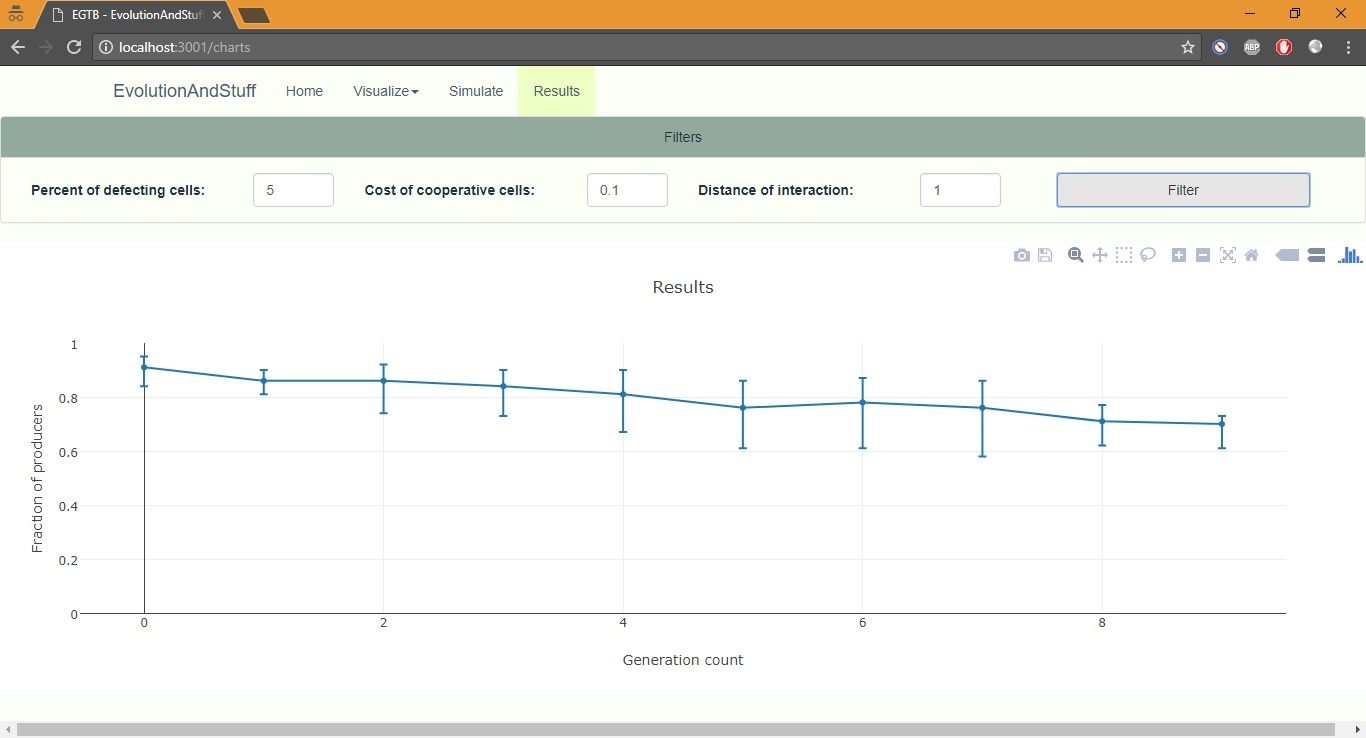
\includegraphics[width=90mm]{images/SimulationResults}
	\caption{Eddigi szimulációk eredményei}
	\label{fig:SimulationResults}
\end{figure}


\section{Felhasznált technológiák}

Már a projekt kezdetekor biztosak voltunk benne, hogy egy könnyen és bárki által elérhető alkalmazásra lesz szükség, így nem volt kérdéses az, hogy webes felületet akarunk. Ezután már csak az volt a kérdéses, hogy számunkra milyen környezet lenne a legkényelmesebb, amely ha szükség van rá könnyen skálázható is. Végül a \textbf{NodeJS}-re (\cite{soft:node}) esett a választásunk, hiszen ez egy egyszerű felület skálázható hálózati alkalmazások írására, valamint egy nagyon egyszerű és elterjedt nyelvet használ, a JavasSriptet. Keretrendszernek a sokak által ismert és használt \textbf{ExpressJS}-t (\cite{soft:express}) választottuk.

Tehát a szoftver egy szerverből és egy kliensből áll, melyek közötti kommunikáció a már jól megszokott HTTP-vel folyik. A fejlesztés során bizonyos szimulációs adatok JSON-beli küldözgetése túl nagy feladatnak bizonyult, így ezek átvitelét \textbf{WebSocket} segítségével oldottuk meg.

%A szerver oldalon folyik az erőforrás igényes számítások nagy része.

Említettük, hogy \textbf{Voronoi} diagramokkal ábrázoljuk a sejteket, így szükségünk volt egy Voronoi modulra is (\cite{soft:voronoiModule}). Ez a modul egy JavaScript implementációja Steven J. Fortune algoritmusának, mely hatékonyon dolgozik Voronoi diagramokkal, viszont csak az adatszerkezettel foglalkozik, nem képes ki is rajzolni azt.

Kliens oldalon a technológiák felhozatala eléggé változatos. Először is egy weboldal jól kell kinézzen és ezen feladatot a \textbf{Bootstrap} (\cite{soft:bootstrap}) keretrendszer tökéletesen ki is elégíti. Dinamikus oldalt lehet vele létrehozni, bármilyen eszközt együttesen lehet kezelni vele, nem csak desktopon de mobil eszközökön is jól néz ki az oldal. Kezdetben kliens oldalon nem nagyon volt bármiféle struktúra a JavaScriptben és elég hamar rá is jöttünk, hogy ez egy hatalmas probléma, a kód elég hamar átláthatatlan lett. Ezért átálltunk \textbf{AngularJS}-re (\cite{soft:angular}), mellyel már sokkal olvashatóbb kódot sikerült létrehoznunk, egyszerűbbé tette a kód bővítését is és az oldal dinamikussága is nőtt (pl. megjelentek az alertek). A Voronoi diagram megjelenítéséért a \textbf{Paper.js} (\cite{soft:paper}) a felelős, valamint itt is jelen van a Voronoi adatszerkezetet feldolgozó modul (\cite{soft:voronoiModule}). A grafikonok kirajzolására több keretrendszert is használunk. Ez azért van mert ismertünk már egyet ami az adott feladatot kielégítette, viszont a későbbiekben új típusú diagramok jöttek be, melyekhez, mint kiderült, új keretrendszerre volt szükségünk. Így alakult, hogy a Voronoi diagram alatti grafikont a \textbf{Highcharts} (\cite{soft:highcharts}) segítségével, a V és g függvényeket (\ref{fig:SimulationFunctionDiagrams}) az AngularJS grafikonjaival, míg az error bart (\ref{fig:SimulationResults}) a \textbf{Plotly.js} (\cite{soft:plotly}) segítségével rajzoltuk ki.

Mivel ez az egész egy webalkalmazás szükségünk volt egy szerverre, ahova ezt kitelepíthetjük. Míg régen ez egy saját szerverre telepítették mely egy statikus IP címmel rendelkezett, addig mára már sokkal könnyebb ha ezt inkább egy felhőbe rakjuk. Több ingyenesen használható felhő is létezik már, a mi választásunk a \textbf{Heroku} lett (az alábbi linken érhető el az alkalmazásunk: \url{https://egtib.herokuapp.com/}). A Heroku egy PaaS típusú felhőszolgáltató, ami annyit jelent, hogy platformot és kész szolgáltatásokat nyújt. Elég volt csak azt megmondani, hogy egy NodeJS alapú szervert akarunk üzemeltetni, ahhoz kiválasztottunk egy akármilyen adatbázist, és már kész is. Természetesen senki sem szereti a kitelepítést kézzel elvégezni, ezért, és persze még sok más hasznos funkcióért is, automatizáltuk a fejlesztést a \textbf{TravisCI} (\cite{soft:travis}) segítségével. A TravisCI egy folytonos integrációs platform, mely könnyen összeköthető github projektekkel, és minden egyes alkalmazás frissítéskor képes előre megadott parancsokat elvégezni. Továbbá ha az alkalmazásunkat egy \textbf{Docker}-be (\cite{soft:docker}) rakjuk, akkor biztosíthatjuk azt, hogy bárhova is kerül az alkalmazásunk, mindig ugyanazon körülmények között fog futni.

Semmilyen kódot nem adhatunk ki a kezünkből, ha annak minősége nincs valahogyan biztosítva. Ezt a minőséget tesztekkel lehet valamilyen szinten biztosítani, amit is megpróbáltunk. Köszönhetően a TravisCI-nak a tesztelés beépítése a fejlesztési folyamatba könnyen ment. Minden egyes új verzió felkerülésekor a github repositoryba, a Travis lefuttatja a teszteket és jelezi, hogy ezek között van-e olyan amely megbukott, illetve rak egy zöld pipát ha mind átment. A unit tesztjeinket a \textbf{Mocha} (\cite{soft:mocha}), míg az E2E tesztjeinket a \textbf{TestCafe} (\cite{soft:testcafe}) keretrendszerekben íródtak. Ezek közül kiemelném a TestCafet, mert ez egy olyan keretrendszer melynél nincs szükség böngésző driverre, egyenesen egy előre telepített böngészőt használ, illetve fel lehet venni vele kattintásokat, azaz ki lehet vele generálni a tesztesetet és nem kell hozzá kódot írni.

\begin{figure}[ht!]
	\centering
	\includegraphics[width=\linewidth]{images/Architecture}
	\caption{A projekt architektúrája\label{fig:Architecture}}
\end{figure}
